\documentclass[12pt]{jarticle}
\usepackage[dvipdfmx]{graphicx}
\usepackage{url}
\usepackage{listings,jlisting}
\usepackage{ascmac}
\usepackage{amsmath,amssymb}

%ここからソースコードの表示に関する設定
\lstset{
  basicstyle={\ttfamily},
  identifierstyle={\small},
  commentstyle={\smallitshape},
  keywordstyle={\small\bfseries},
  ndkeywordstyle={\small},
  stringstyle={\small\ttfamily},
  frame={tb},
  breaklines=true,
  columns=[l]{fullflexible},
  numbers=left,
  xrightmargin=0zw,
  xleftmargin=3zw,
  numberstyle={\scriptsize},
  stepnumber=1,
  numbersep=1zw,
  lineskip=-0.5ex
}
%ここまでソースコードの表示に関する設定

\title{知能プログラミング演習II 課題3}
\author{グループ8\\
  29114003 青山周平\\
}
\date{2019年11月5日}

\begin{document}
\maketitle

\paragraph{提出物} rep3
\paragraph{グループ} グループ8
\paragraph{メンバー}
\begin{tabular}{|c|c|c|}
  \hline
  学生番号&氏名&貢献度比率\\
  \hline\hline
  29114003&青山周平&null\\
  \hline
  29114060&後藤拓也&null\\
  \hline
  29114116&増田大輝&null\\
  \hline
  29114142&湯浅範子&null\\
  \hline
  29119016&小中祐希&null\\
  \hline
\end{tabular}



\section{課題の説明}
\begin{description}
\item[必須課題3-1] セマンティックネットのプログラムを参考に,グループメンバー全員(およびその周辺人物)についてのセマンティックネットを構築せよ.
個人レポートには自分のみ(とその周辺)に関するセマンティックネットを示し,グループレポートには全員(とその周辺)に関するセマンティックネットを示せ.
\item[必須課題3-2] フレームのプログラムを参考に,自分達の興味分野に関する知識をフレームで表現せよ.その分野の知識を表す上で必須となるスロットが何かを考え,クラスフレームを設計すること.
個人レポートには自分が作ったインスタンスフレームのみ(クラスフレームの設計担当者はクラスフレームも)を示し,グループレポートにはクラスフレームおよび全員分のインスタンスフレームを示せ.
\item[必須課題3-3] 課題3-1または3-2で作った知識表現を用いた質問応答システムを作成せよ.
なお,ユーザの質問は英語や日本語のような自然言語が望ましいが,難しければ課題2で扱ったような変数を含むパターン (クエリー) でも構わない. 
\item[発展課題3-4] 課題3-1または3-2で作った知識表現を図として示すためのユーザインターフェース(GUI) を設計し実装せよ.
\item[発展課題3-5] 上記3-3で作成した質問応答システムを,DBpediaあるいはWikidata中の知識を使って質問に答えられるよう,拡張せよ.
\end{description}

\section{必須課題3-1}
\begin{screen}
セマンティックネットのプログラムを参考に,グループメンバー全員(およびその周辺人物)についてのセマンティックネットを構築せよ.

個人レポートには自分のみ(とその周辺)に関するセマンティックネットを示し,グループレポートには全員(とその周辺)に関するセマンティックネットを示せ.
\end{screen}
私(とその周辺)に関するセマンティックネットの構造は,下図の通りである.
\begin{figure}[!hbt]
  	\begin{center}
	\end{center}
  	\caption{セマンティックネット}
\end{figure}


\section{必須課題3-2}
\begin{screen}
フレームのプログラムを参考に,自分達の興味分野に関する知識をフレームで表現せよ.その分野の知識を表す上で必須となるスロットが何かを考え,クラスフレームを設計すること.

個人レポートには自分が作ったインスタンスフレームのみ(クラスフレームの設計担当者はクラスフレームも)を示し,グループレポートにはクラスフレームおよび全員分のインスタンスフレームを示せ.
\end{screen}
私が作ったインスタンスフレームは下図のような設計となっている.
\begin{figure}[!hbt]
  	\begin{center}
  		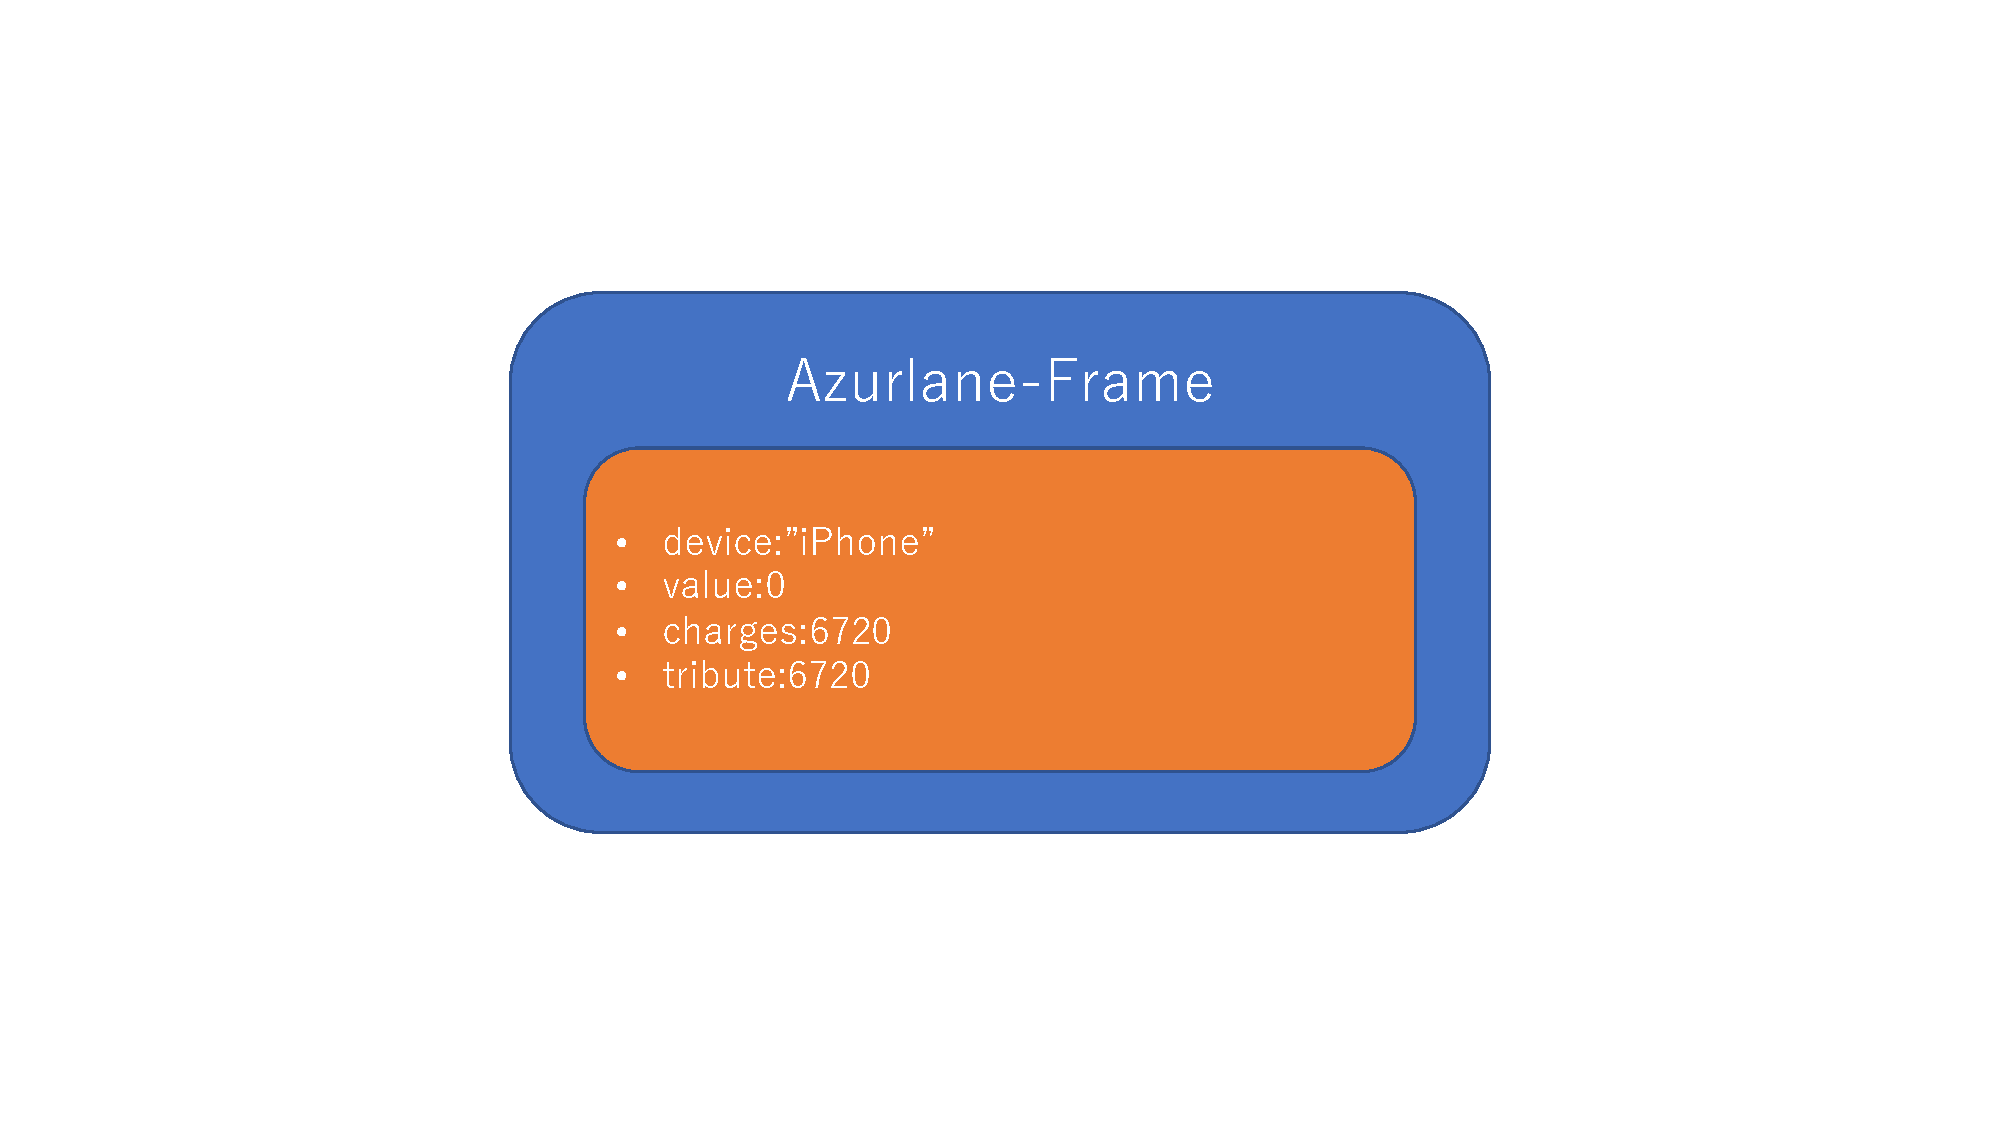
\includegraphics[scale=0.40]{images/azurlane.pdf}
	\end{center}
  	\caption{インスタンスフレーム}
\end{figure}



\section{必須課題3-4}
\begin{screen}
課題3-1または3-2で作った知識表現を図として示すためのユーザインターフェース(GUI) を設計し実装せよ.
\end{screen}
私の担当箇所は,発展課題3-4におけるGUIのSwingを用いた実装である.

\subsection{手法}
セマンティックネットのためのGUIを実装するにあたり,以下のような方針を立てた.
\begin{enumerate}
\item ノードやリンクのデータを受け取る.
\item ノードを表示するためのパネルを作り,リンクを表示するための描写を設定する.また,パネルをマウスで移動できるようにする.
\item 検索・追加・削除の機能を追加する.
\end{enumerate}

1.に関して,表示するコンポーネントを,オリジナルのクラスを用いて階層的に管理することで,より拡張性・保守性の高い管理しやすいプログラムとなるよう心がけた.

2.に関して,セマンティックネットのような複雑な図をユーザが自身で最も見やすい表示にするために,マウスによるドラッグでパネルを移動できるような仕様とした.

3.に関して,これらの機能をセマンティックネットとは別のパネルに分けたことで,より構造化されたGUIとなるようにした.

また,セマンティックネットのGUIを元にして,フレームのGUIも作った.

\clearpage

\subsection{実装}
セマンティックネットのGUIに関するプログラムSemNetGUI.javaには以下のクラスが含まれる.
\begin{itemize}
\item SearchGUI: メソッドmain, actionPerformed, クラスmyListenerを実装したクラス.
\item View: インターフェースViewInterfaceを実装したメソッド,各種ゲッターを実装したクラス.
\end{itemize}

フレームのGUIに関するプログラムFrameGUI.javaには以下のクラスが含まれる.
\begin{itemize}
\item SearchGUI: メソッドmain, actionPerformed, クラスmyListenerを実装したクラス.
\item View: インターフェースViewInterfaceを実装したメソッド,各種ゲッターを実装したクラス.
\end{itemize}

\subsubsection{ノードやリンクのデータを受け取る}
AccessData.javaを介する

\subsubsection{ノードを表示するためのパネルを作り,リンクを表示するための描写を設定する.また,パネルをマウスで移動できるようにする}

\subsubsection{検索・追加・削除の機能を追加する}

\subsubsection{セマンティックネットのGUIを元にして,フレームのGUIを作る}


\clearpage
\subsection{実行例}
UnifyGUIを実行したところ,下図のような画面が得られる.

\begin{figure}[!hbt]
  	\begin{center}
	\end{center}
  	\caption{初期状態}
\end{figure}
\clearpage


\subsection{考察}


\section{感想}


% 参考文献
\begin{thebibliography}{99}
TATSUO IKURA: 『Swingを使ってみよう - Java GUIプログラミング』 https://www.javadrive.jp/tutorial/ (2019/10/29アクセス) \\
\end{thebibliography}

\end{document}
